\documentclass{article}

\usepackage[final]{nips_2017}

\usepackage[utf8]{inputenc} % allow utf-8 input
\usepackage[T1]{fontenc}    % use 8-bit T1 fonts
\usepackage{hyperref}       % hyperlinks
\usepackage{url}            % simple URL typesetting
\usepackage{booktabs}       % professional-quality tables
\usepackage{amsfonts}       % blackboard math symbols
\usepackage{nicefrac}       % compact symbols for 1/2, etc.
\usepackage{microtype}      % microtypography

\usepackage{algorithm}
\usepackage{algorithmic}

\usepackage{amsmath}
\DeclareMathOperator*{\argmax}{arg\,max}

\usepackage{graphicx}
%\graphicspath{ {./} }
\usepackage{wrapfig}

\title{Deep Q-learning in OpenAI gym}

\author{
  Renat Aksitov\\
  \texttt{raksitov@stanford.edu} \\
}

\begin{document}

\maketitle
\begin{abstract}
  Since Deepmind published the first paper [1] on applying deep reinforcement learning for training an agent that plays Atari games, many additional enhancements for the original DQN algorithm were proposed. In this project I will explore some of these improvements and will measure their impact on the overall training performance.
\end{abstract}

\section{Introduction}

In the reinforcement learning the goal is to train the agent based solely on a sensory input, which potentially could be very high-dimensional. The algorithm used by such agent should be generic and having as little assumptions about specific problem at hand as possible. To satisfy these conditions it is feasible to use OpenAI Gym [3] as a training facility. OpenAI Gym is a reinforcement learning benchmark that provides large (and growing) set of different tasks (POMDPs called \emph{environments}). Environments share common interface and are versioned, which keeps results reproducible over time. Examples of the available environments include classic control and toy text problems from RL literature, sets of Atari and board games etc.

For my experiments in this project I am focusing on a classic CartPole environment [4]. It's worth noting that this environment, due to its simplicity, could be solved by much less sophisticated methods than reinforcement learning - like random search or hill climbing, for example. The main point of choosing CartPole for experiments is that, unlike Atari environments, it allows to perform a lot of trials with moderate computational resources. In the same time, most of the results observed for CartPole, should still be applicable to other, more complex environments. One important difference is that while Atari games have sparse rewards, CartPole has dense rewards. I am describing some implications of this in the "Experiments" section \ref{Experiments}.

I am starting my experiments from the basic deep Q-learning algorithm and then expanding it with various tweaks like \emph{experience replay} and {\it target networks}.

\section{Related work}
This project is primarily based on the work done by Deepmind recently. Before 2013, most of the reinforcement learning publications were focusing on linear function approximators, due to them having much better theoretical convergence guarantees than nonlinear ones [5]. This changed after Deepmind has successfully applied deep Q-learning (DQN) to solving 7 Atari games with super-human performance on 3 of them [1]. Arguably, the main innovation in this work was introduction of the experience replay, which helps to stabilize the algorithm. With the experience replay, instead of training on the batch of the most recent experiences, which are all highly correlated, we first put all the experiences into memory buffer and then train on a random sample from this buffer. Some other tricks in [1] include skipping frames and preprocessing of the input to reduce its dimensionality, as well as stacking 4 last frames together to provide model with the dynamic picture. The paper also suggests that it might be worthwhile to use another sampling strategy for the experience replay. [6] explores this idea further and develops approach to replay important experiences more frequently, and therefore learn more efficiently.

    In 2015 Deepmind published follow-up [2] for the original paper from 2013. In it they extended training set to 49 Atari games and added several additional enhancements to the algorithm, including gradient clipping and introducing of a second deep network. This second target network is only occasionally updated with the values from the main Q-network, with the goal to reduce correlations of the action-values with the target values. In yet another paper from Deepmind [7], instead of updating target network periodically every C steps, they are using "soft" updates, so that weights of the target network are slowly updated towards the weights of the Q-network. This modification aims to improve the stability of the learning with the target network.

    It is known that original DQN algorithm tends to overestimate action values, due to using the same values both to select and to evaluate an action. This problem is addressed by the double Q-learning algorithm (DDQN), introduced in [8]. The idea behind DDQN is to use the Q-network for evaluation and the target network for action selection. This way the target network is not completely decoupled from the main network, but the change from DQN algorithm to DDQN is minimal.
    
     Finally, [9] combines many of the extensions mentioned above (and some others, like, for example, dueling networks [10] and multi-step learning [11]) into the Rainbow model, which significantly outperforms each of its components. The authors did an ablation study, which shows that the only component without performance benefits for the final Rainbow model was dueling networks.

\section{Background}

\subsection{Reinforcement learning}
Following [1], I am considering standard RL setup in which an agent interacts with an environment $\mathcal{E}$ in a sequence of {\it actions}, {\it observations} and {\it rewards}. During one step of an interaction an agent selects an action from a set of all possible actions $\mathcal{A}=\{1,K\}$, which does not change with time. This action is passed to the environment, the internal state of the environment is changed (possibly, stochastically) and an observation $s_t$ and reward $r_t$ are returned to the agent. The end goal of an agent is to select actions in a way that maximizes future rewards. Let's calculate the full reward from time $t$ as a standard {\it discounted} reward with discount $\gamma$:
\begin{equation}\label{eq:reward}
R_t = r_t + \gamma r_{t+1} + \gamma^2 r_{t+2} + ...
\end{equation}
We could now define an optimal action-value function as a maximum expected reward that could be achieved by following the best policy after seeing some state $s$ and taking some action $a$:
\begin{equation}\label{eq:Q}
Q^*(s,a) = \max_{\pi}\mathbf{E}[R_t|s_t=s,a_t=a,\pi]
\end{equation}
It is well known that an optimal policy should satisfy {\it Bellman} equation. This allows us to apply Bellman equation iteratively to estimate action-value function:
\begin{equation}\label{eq:Bellman}
Q_{i+1}(s,a) = \mathbf{E}_{s'}[R + \gamma \max_{a'} Q_i(s',a')|s,a]
\end{equation}

\subsection{DQN}
Value iteration \ref{eq:Bellman} is guaranteed to converge to an optimal Q-function, but it is not very practical as is, without any generalization. The common approach to fix this is by using {\it function approximator} $Q(s, a, \theta) \approx Q^*(s,a)$. [1] suggests to use deep neural network as a function approximator and calls such an approximator a Q-network. Parameters $\theta_i$ in this case are weights of the deep network in the i-th iteration and the loss of the Q-learning update could be written as follows:
\begin{equation}\label{eq:Loss}
L_i(\theta_i) = \mathbf{E}_{(s,a,r,s') \in D}[r + \gamma \max_{a'}Q(s', a', \theta_{i-1}) - Q(s, a, \theta_i)]
\end{equation}
Instead of calculating a full expectation, it is much less computationally expensive to optimize the loss \ref{eq:Loss} via stochastic gradient descent. In this subsection, the step of the gradient descent is applied on the minibatch of the most recent consecutive experiences $(s, a, r, s')$, this will change after introduction of the experience replay.

Value iteration is {\it off-policy} algorithm, meaning that at every iteration $i$ the current estimate of the Q-function $Q(s, a, \theta_i)$ is used to select the next action by following a greedy strategy: $a = \argmax_{a'}Q(s,a',\theta_i)$. More precisely, our strategy will actually be $\epsilon$-greedy, to ensure the proper exploration of a state space: e.g., the next action will be chosen greedily with probability $1 - \epsilon$ and randomly with probability $\epsilon$. By putting it all together, we are getting the DQN algorithm in its simplest form.

\begin{algorithm}[H]
\caption{Deep Q-learning algorithm}
\label{alg1}
Initialize action-value function Q with random weights $\theta$.
\begin{algorithmic}
\FOR{($episode=1$ to $M$)}
\STATE Initialize start state $s_1$.
\FOR{($t=1$ to $T$)}
\STATE With probability $\epsilon$ select a random action $a_t$,
\STATE otherwise select $a_t = \argmax_{a}Q(s,a,\theta)$.
\STATE Execute action $a_t$ in the environment and observe reward $r_t$ and new state $s_{t+1}$.
\STATE Add transition $(s_t, a_t, r_t, s_{t+1})$ to the buffer D.
\IF{($length(D) >= minibatch$)}
\STATE Choose $minibatch$ of the most recent transitions from D, $j\in1..minibatch$.
\STATE Set $y_j = \begin{cases} r_j, & \mbox{if episode terminates at step j + 1,} \\ r_j + \gamma \max_{a'}Q(s_{j+1}, a', \theta), & \mbox{otherwise.} \end{cases}$
\STATE Perform a gradient descent step on $(y - Q(s, a, \theta))^2$ with respect of the weights $\theta$.
\ENDIF
\ENDFOR
\ENDFOR
\end{algorithmic}
\end{algorithm}

Note that the resulting algorithm is {\it model-free} - it uses samples from the environment directly, without trying to estimate rewards and transitions dynamics.

\subsection{Environment}

\begin{wrapfigure}{r}{0.33\textwidth} %this figure will be at the right
    \centering
    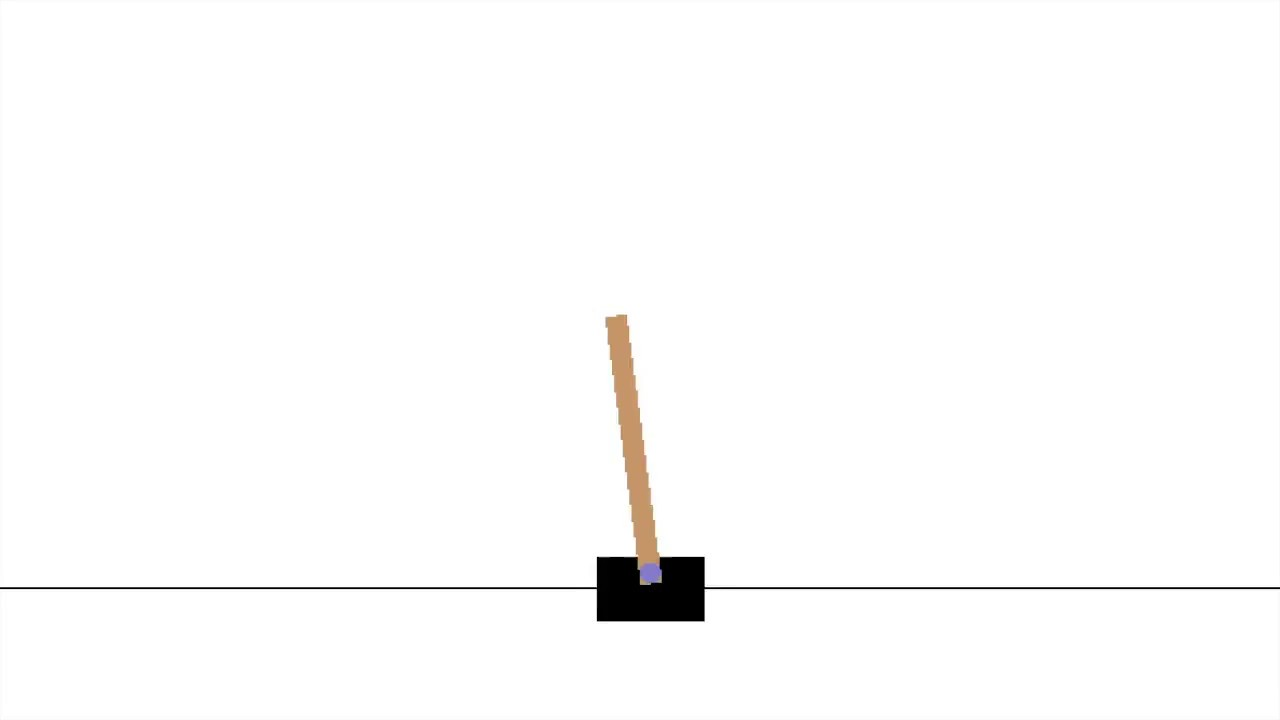
\includegraphics[width=0.25\textwidth]{cartpole}
    \caption{CartPole environment.}
\end{wrapfigure}

Interacting with any Gym environment is straightforward. First, we create the environment object from the name of the particular environment and its version (for example, 'CartPole-v0'), then we reset it to get a start state of an episode. After that we can invoke step() method with a specific action we would like to take and it will change internal state to the next one, as well as return a new observation, a reward and whether an episode has terminated after this step. The environment object could also be used to get an auxiliary information (like size of an action space, for example) and for rendering the episode in the video form.

My experiments are done for the CartPole environment [4], which has just 2 actions (push cart to the right or to the left) and a 4-dimensional observation space consisting of a cart position and velocity, a pole angle and a pole velocity at a tip. Every step until termination we receive a unit of reward and the goal is to terminate as late as possible. This environment is considered "solved" if average reward over 100 consecutive episodes is at least 195 (out of 200 maximum) for v0 and 475 (out of 500) for v1.

\subsection{Extensions}
I will try the following extensions for the base DQN algorithm.
\begin{itemize}
  \item {\bf Experience replay}. Instead of training gradient descent on the most recent experiences, we could uniformly sample the minibatch of experiences from the whole memory buffer D.
  \item {\bf Target network}. The idea is to use a separate network for estimating value of a target $y_j$. More specifically, every C steps we will copy main Q-network into a separate target network $\overset{\wedge}{Q}$ with weights $\theta^-$ and use it to estimate $y_j$ during the following C steps. An update after this change could be written like this:
\begin{equation}\label{eq:target}
r + \gamma \max_{a'}\overset{\wedge}{Q}(s', a', \theta^-_i) - Q(s, a, \theta_i)
\end{equation}
  \item {\bf Gradient clipping}. This was originally suggested in [2]. We just clip the error term of an update \ref{eq:target} to be between -1 and 1.
  \item {\bf Continuous updates}. Instead of copying the main network Q into target network $\overset{\wedge}{Q}$ every C steps, let's change the target network weights $\theta^-$ into the weights $\theta$ of the main network during each step but slowly. E.g. by applying $\theta^- \leftarrow \tau \theta + (1 - \tau) \theta^-$ with $\tau \ll 1$.
  \item {\bf Double network}. This enhancement tries to reduce overestimation by decomposing taking maximum in the $y_j$ into action selection and action evaluation. The update \ref{eq:target} for the double network will take the following form:
\begin{equation}\label{eq:double}
r + \gamma \overset{\wedge}{Q}(s', \argmax_{a}Q(s',a,\theta_i), \theta^-_i) - Q(s, a, \theta_i)
\end{equation}  
\end{itemize}

\section{Experiments}
\label{Experiments}

\subsection{Implementation}
Unlike [1], that uses multilayered convolutional network, I am defining 1-layer deep feed-forward network as an approximator, which is enough for CartPole and significantly reduces training time. Also unlike [1], I am optimizing loss via GradientDescent optimizer instead of RMSprop, to simplify hyperparameters tuning. To make this optimizer somewhat adaptive, I am applying linear decay to its learning rate. I have found that, at least for CartPole, it's beneficial to use the decay with respect to the current average reward, rather than to decay with time as [1] does. The idea here is to reduce learning rate when average reward becomes close to the target reward and to increase it back if the average reward falls significantly. I am applying the same decay to $\epsilon$ that defines random exploration. Note, that linear decay of this form exploits dense rewards of CartPole and it is unlikely to work well in cases with sparse rewards, like Atari.

\subsection{Results}
Similar to [1], I am measuring average reward (over 100 episodes, so it is consistent with environment's definition of being "solved") and average predicted action-value as performance metrics. To calculate the latter, before starting training I am running random policy for 1000 observations and choosing 10 states from them (states should be fairly spaced from each other, so that they are not correlated). These 10 states are then used to periodically calculate the average predicted action-value.

I have run my experiments on v1 version of the CartPole. The results are presented on the figures 2 - 5 (4 letter encoding of the curves corresponds to the DQN extensions that are enabled or disabled for this particular curve; for example "RTND" for orange on figure 4 means that this curve has experience replay, target and double network enabled and continuous update disabled). There are several things worth noting here:
\begin{itemize}
\item {\bf Baseline}. Purely random strategy achieves average reward of $\sim 20$. This is about 50\% higher, than the average reward when training diverges ($\sim 13$). The divergence could happen either due to the bad choice of hyperparameters or due to unlucky random initialization of Q-network. The example of the latter is an "orange" curve shown on the figure 4.
\item {\bf Extensions comparison}. From figure 3 we can see that in the absence of experience replay target network (dark blue) achieves significant improvement over basic DQN algorithm (orange), but adding continuous updates or double network slightly decreases performance. Now compare with figure 4. The experience replay by itself (green) starts to converge faster than basic algorithm from previous figure, but is unstable without target network. At the same time, the brown  algorithm with all 4 extensions enabled demonstrates superior performance to everything else and the only one that "solves" the environment within the limit of 100K episodes.
\item {\bf Gradient clipping}. I have noticed very early that it does not work for CartPole (network can not get much above random baseline, see figure 5), so it is not present in ablation experiments. The most likely cause for this mismatch with [2] are dense rewards of the CartPole, but it is unclear for me how to prove it.
\item {\bf Smooth rewards}. The plots of average rewards from figure 3 and 4 are much smoother than plots of average predicted Q-values from figure 2. This is actually exactly opposite of what was reported in [2]! What's the reason for this switch? Turns out, it is the lack of gradient clipping. Compare with curves smoothness on figure 5.

  Another thing to note from figure 2 is how smoothness of Q-function increases from base algorithm (orange) after adding target network (blue) and experience replay (gray). Finally, brown with all extensions enabled seems to have the most smooth Q-function.
\end{itemize}

\begin{figure}[h]
    \centering
    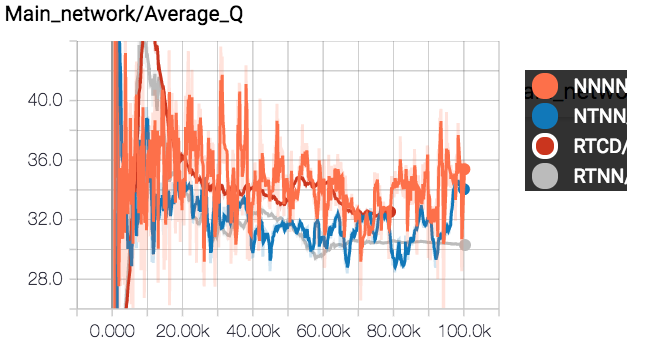
\includegraphics[width=\textwidth]{QPlotFixed}
    \caption{Average predicted action-value for CartPole-v1 (letter coding: "R" - experience replay, "T" - target network, "C" - continuous update, "D" - double network, "N" - base case, absense of a feature).}
\end{figure}

\begin{figure}[h]
    \centering
    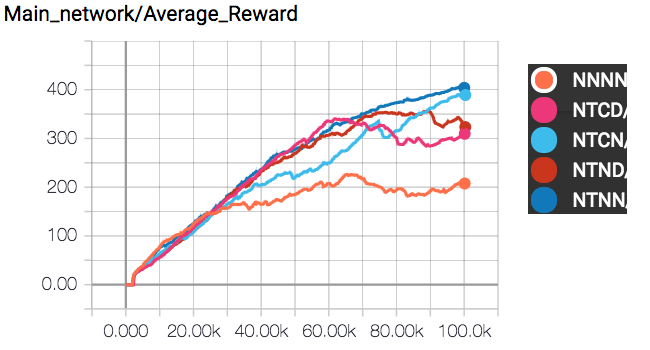
\includegraphics[width=\textwidth]{BPlotFixed}
    \caption{Average Reward for CartPole-v1 without experience replay (letter coding: "R" - experience replay, "T" - target network, "C" - continuous update, "D" - double network, "N" - base case, absense of a feature).}
\end{figure}

\begin{figure}[h]
    \centering
    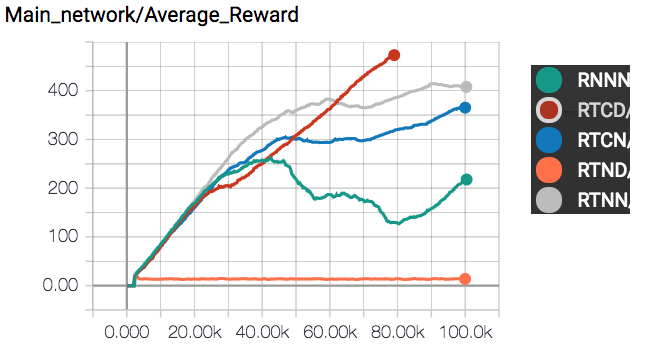
\includegraphics[width=\textwidth]{RPlotFixed}
    \caption{Average Reward for CartPole-v1 with experience replay (letter coding: "R" - experience replay, "T" - target network, "C" - continuous update, "D" - double network, "N" - base case, absense of a feature).}
\end{figure}

\begin{figure}[h]
    \centering
    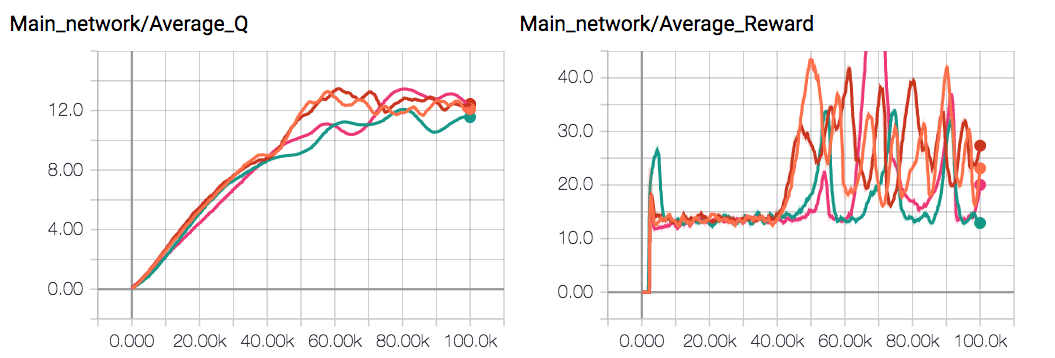
\includegraphics[width=\textwidth]{gradient}
    \caption{Average Reward and Q-function for CartPole-v1 with gradient clipping.}
\end{figure}

\section{Conclusions}
I have successfully applied DQN algorithm to OpenAI Gym CartPole environment. I also did an ablation study and have found that 4 out of 5 considered extensions provide clear performance benefits (experience replay, target network, continuous update and double network). The last extension, gradient clipping, does not allow the algorithm to converge on the CartPole environment.

{\it The code is available in \url{https://github.com/raksitov/rl-in-openai-gym}.}

\section*{References}

[1] Mnih, V., Kavukcuoglu, K., Silver, D., Graves, A., Antonoglou, I., Wierstra, D. and Riedmiller, M., 2013. {\bf Playing atari with deep reinforcement learning}. {\it arXiv preprint arXiv:1312.5602}.

[2] Mnih, V., Kavukcuoglu, K., Silver, D., Rusu, A.A., Veness, J., Bellemare, M.G., Graves, A., Riedmiller, M., Fidjeland, A.K., Ostrovski, G. and Petersen, S., 2015. {\bf Human-level control through deep reinforcement learning}. {\it Nature, 518(7540), pp.529-533}.

[3] Brockman, G., Cheung, V., Pettersson, L., Schneider, J., Schulman, J., Tang, J. and Zaremba, W., 2016. {\bf OpenAI gym}. {\it arXiv preprint arXiv:1606.01540}.

[4] \url{https://github.com/openai/gym/wiki/CartPole-v0}

[5] John N Tsitsiklis and Benjamin Van Roy. {\bf An analysis of temporal-difference learning with function approximation}. {\it Automatic Control, IEEE Transactions on, 42(5):674–690}, 1997.

[6] Schaul, T., Quan, J., Antonoglou, I. and Silver, D., 2015. {\bf Prioritized experience replay}. {\it arXiv preprint arXiv:1511.05952}.

[7] Lillicrap, T.P., Hunt, J.J., Pritzel, A., Heess, N., Erez, T., Tassa, Y., Silver, D. and Wierstra, D., 2015. {\bf Continuous control with deep reinforcement learning}. {\it arXiv preprint arXiv:1509.02971}.

[8] Van Hasselt, H., Guez, A. and Silver, D., 2016, February. {\bf Deep Reinforcement Learning with Double Q-Learning}. {\it In AAAI (pp. 2094-2100)}.

[9] Hessel, M., Modayil, J., Van Hasselt, H., Schaul, T., Ostrovski, G., Dabney, W., Horgan, D., Piot, B., Azar, M. and Silver, D., 2017. {\bf Rainbow: Combining Improvements in Deep Reinforcement Learning}. {\it arXiv preprint arXiv:1710.02298}.

[10] Wang, Z., Schaul, T., Hessel, M., Van Hasselt, H., Lanctot, M. and De Freitas, N., 2015. {\bf Dueling network architectures for deep reinforcement learning}. {\it arXiv preprint arXiv:1511.06581}.

[11] Sutton, R.S. and Barto, A.G., 1998. {\bf Reinforcement learning: An introduction} (Vol. 1, No. 1). {\it Cambridge: MIT press}.

\end{document}